\section{Proposed Design Architecture}
\label{sec:Solution}
In this section, we describe the system architecture and design choices we made. 

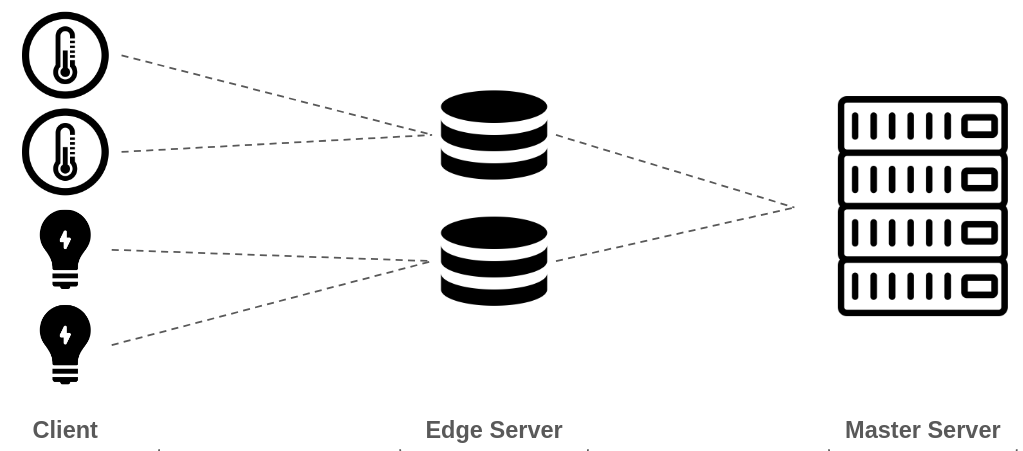
\includegraphics[width=10cm, height=5cm]{sections/Figures/architecture.png}

\subsection{Client}

Client has a local data store which periocially 

\subsection{Edge Server}
We implemented our own key-value format database which edge-server inherits from. We define three main queries for read, write, and update. Edge server is meant to be close to the clients and we deployed a REST API for connection between clients and edge servers. The main functionality of edge server is to authorize clients and execute their queries on database and return the result. Since we used REST API, we used \texttt{Put} for write query, \texttt{Get} for read query and \texttt{Delete} for delete query.


\subsection{Master Server}
It's important that we guarantee the data persistence among edge servers. We need to make sure if edge servers crashed we don't lost access to it's database; therefore, we also implemented master servers.
Master servers receive backup files from the edge servers and store them in a secure, permanent disk storage. Since, there might be a similar key being used by different edge servers, master-server does not translate backup files into a database object and store them as a \texttt{json} file.
